\projectname~(\projectmeaning) is our realization of the techniques described in
\S\ref{sec:approach}. \projectname~is implemented in roughly 10,000 lines of Python in
addition to the Hassel network invariant checking library~\cite{hsa}. The code
for \projectname~is publicly available,\footnote{URL omitted due to anonymity requirements}
and three industrial SDN companies have expressed interest in adopting it.\colin{Cite?}

In the rest of this section, we highlight salient points of \projectname's
design. Furthermore, we describe three ways \projectname~can be put to use
by SDN developers and operators.

The input types supported by \projectname~are shown in Table~\ref{tab:inputs}.
Controllers are notified of link, switch, and host migration events
via OpenFlow messages~\cite{openflow} sent by software switches.
Although the software switches do support packet forwarding, we
have chosen to de-emphasize dataplane performance in favor of
being able to simulate networks of large sizes. % as we show in \S\ref{subsec:runtime}.
% We hope to support policy changes in the future (Quantum)

\begin{table}
\centering
\begin{tabular}{|l|l|}
\hline
Link failure & Link recovery \\
\hline
Switch failure & Switch recovery \\
\hline
Control server failure & Control server recovery \\
\hline
Dataplane packet injection & Host migration \\
\hline
Control message delay & \\
\hline
\end{tabular}
\caption{Input types supported by \projectname}
\label{tab:inputs}
\end{table}

We designed \projectname~to be as resilient to non-determinism as possible
while minimizing modifications to control software.
\projectname ensures a deterministic order of messages despite
non-determinism in operating system I/O scheduling
by multiplexing all sockets in the controller process
onto a single true socket. \projectname~currently
overrides socket functionality within the control software itself, but
deterministic I/O could also be achieved without code modifications by
loading a shim layer on top of
libc (similar to liblog~\cite{Geels:2006:RDD:1267359.1267386}).

With a
small change to the control software's logging library \projectname~can be
notified whenever a log statement is executed,
and thereby account for relevant internal state changes while scheduling inputs.
Routing {\tt gettimeofday()} and {\tt getrand()} through
\projectname~makes replay more resilient to alterations in execution
speeds.\footnote{When the pruned trace differs from the original, we make a
best-effort guess at what the return values of these calls should be. For example,
if the altered execution invokes {\tt gettimeofday()} more times than were recorded
in the initial run, we interpolate the time values of neighboring events}
As an added benefit, overriding {\tt gettimeofday()} allows us to `compress'
runtime in some cases (similar to~\cite{Gupta06toinfinity}).

\projectname~can be used in a number of ways. We outline three use-cases here.

\subsection{Testing}

\projectname~is primarily used as a simulation and testing framework.
With complete control over event orderings, message drops, node
failures, \etc, \projectname~is especially useful for exploring corner cases
and ``what if'' questions. Along these lines, Amin Vahdat
has testified to the value of Google's SDN network simulator~\cite{vadhat}:
\begin{quote}
``One of the key benefits we have is a very nice emulation and
simulation environment where the exact same control software that would be
running on servers might be controlling a combination of real and emulated
switching devices. And then we can inject a number of failure scenarios under
controlled circumstances to really accelerate our test work.''
\end{quote}

In testing mode, \projectname~generates random or interactively chosen input
sequences, feeds them to controller(s), and monitors invariants at chosen
intervals. Driving the
execution of the system in this way allows \projectname~to record a
totally-ordered log of the events to be replayed later.

As additional failure cases are encountered they can be added
to a suite of integration tests and later used to validate the correct
behavior of future versions of the software. And because \projectname~makes
limited assumptions about the control software under test, the overall SDN community
could collect a repository of test cases to validate different SDN control platforms.

Automatically generating integration tests and identifying
minimal causal sequences frees developers to be more agile in
development, decreasing the time they spend writing test cases,
performing triage, and
hunting bugs. Beyond making test cases easier to reason about, minimal causal
sets serve to consolidate redundant test cases and thereby reduce time wasted
investigating bug reports the same root
cause~\cite{Zeller:2002:SIF:506201.506206}:
if two test failures have the same minimal causal sequence, it is
likely that the same underlying bug is being triggered.

\subsection{Replayable Traces}

When developers are unable to debug an issue, they often elicit help from
mailing lists or coworkers. The status quo today is to describe the conditions needed to
reproduce the bug as carefully as possible and hope that someone else is able
to replicate the issue.

With \projectname, developers can readily record errant executions and
exchange replayable traces with each-other.
Replayable traces shorten the debugging cycle, and increase chances that others
will be able to help. For example, bug reports can be filed with a replayable trace
attached, so that no
effort is wasted replicating the issue. With the help of print statements or a
debugger, developers can also iteratively run the trace as many times as
needed to identify the line(s) of code responsible for the problem.

\subsection{Forensic Analysis}

Perhaps the most valuable use case for \simulator~is forensic analysis of
production logs--correctness violations encountered in production are
high priority, and often time consuming to diagnose. While we have not
implemented this functionality, we present a sketch of
how forensic analysis could be performed with \simulator.

While \simulator~takes as input a single, totally-ordered log of the events in the
distributed system, production systems maintain a log at each node.
Instrumentation and preprocessing steps are therefore needed before \simulator~can be
invoked.

Production systems would need to include Lamport
clocks on each message~\cite{Lamport:1978:TCO:359545.359563} or have
sufficiently accurate clock
synchronization~\cite{corbett2012spanner} to obtain a partial global ordering
consistent with the happens-before relation.
Note that a total ordering is not needed, since it is permissible
for \simulator~to reorder concurrent events from
the production run so long as the happens-before relation is
maintained~\cite{Fischer:1985:IDC:3149.214121}.

The distributed logs would also need to make a clear distinction between internal events
(log messages, message sends/receipts), and input events (\eg~node failures). Further,
the input events would need to be logged in sufficient detail for \simulator~to
reproduce a synthetic version of the input that is indistinguishable to the control software
from the original input event. There will of course be some input events that cannot be reproduced
synthetically without significant complexity in what the simulator needs to model.
For example, suppose that the controller's faulty behavior is to flood a switch with messages,
causing the switch to drop some traffic. Yet only switches that are running low on memory
are affected by the controller's faulty behavior. To reproduce this failure mode correctly,
the simulator would need to model the memory levels of its software switches to match the
hardware behavior exactly.

Without care, a single input event may appear multiple times in the
distributed logs. A failure of the master node, for example, could be independently
detected and logged by all other replicas. The most robust way to
avoid redundant input events is to employ perfect failure
detectors~\cite{chandra1996unreliable}, which have the property that a
failure is logged iff
the failure actually occurred.\footnote{Perfect failure detectors are
typically implemented by explicitly killing slow
nodes.} Ensuring that a single failure detector is in charge of logging node failure
events guarantees that redundant inputs are eliminated. Alternatively, root cause analysis
algorithms~\cite{577079} or manual inspection could be employed to consolidate redundant
alarms.

Finally, some care may need to be taken to prevent the logs from growing so large that
\simulator's runtime becomes intractable. Here, causally consistent
snapshots~\cite{Chandy:1985:DSD:214451.214456} can minimize the number of inputs \simulator~needs
to examine. Specifically, with causally consistent snapshots of the distributed
system taken at regular intervals, \simulator~can bootstrap its simulation from the last snapshot before the failure.
If the MCS starting from this snapshot is empty, it can iteratively move backwards, starting from earlier
snapshots.\footnote{Technically the MCS may contain inputs from the very beginning of the execution. Arguably though,
the state that was induced by these inputs is reflected in each snapshot, and programmers would be able to detect
this by examining that state with a debugger.}

% --------------------------------------------------
%    OLD TEXT

\eat{

\subsubsection{Additional Use-Cases} Besides lifetime tracking and causal analysis, our simulation infrastructure has a
number of other possible use-cases:

\noindent\textbf{Checking related problems by fuzzing.} Input traces can be
\emph{fuzzed}~\cite{Miller:1990:ESR:96267.96279}, \ie{},
randomly perturbed, to expose the system to similar error conditions, and confirm
that a proposed solution is not just a point-fix. \colin{Need to be more clear
about what the constraints on the fuzzer are. (permutation or generation?)}

\noindent\textbf{Investigating pathological environment conditions.} The simulator allows for investigation
of pathological environment conditions difficult to achieve in a real world test bed
(\eg{}, correlated failure rates, extremely long delays etc.). This enables
investigation of situations that have a high potential for triggering errors.

\noindent\textbf{Interactive exploration.} Troubleshooters can also interactively bisect
the trace or modify specific events to further pinpoint the cause for a failure.
This is useful as soon as a suspect event sequence has been identified.

\noindent\textbf{Regression/Integration Test Library.} In traditional software engineering practices,
integration tests are an
important part of the software development cycle: developers feed end-to-end
input through the system, and verify that the system execution satisfies
certain safety and liveness properties. As additional failure cases are encountered in
production, new cases can be added to a suite of integration tests to
ensure robust operation of the system in future versions of the system.

Although the practice of accumulating an integration test suite over time is
commonplace in other fields of computer science, the field of networking
simply did not have the requisite software infrastructure to realize this practice before the emergence
of SDN. \Simulator{} can be viewed as our realization
of this development practice, applied to network controllers. Our simulator's fine-grained control over
failure scenarios allows us to test corner-case network conditions -- those
that are most difficult to anticipate in traditional unit tests.
As known failure cases are accrued over time, we envision \simulator{} being used to validate
new and existing SDN platforms.
}


\eat{

% Research question here?
% Going to be challenging to have this not come across as a software design
% spec.. Let's try to get this section over with as little text wasted as
% possible... I feel silly writing these sections, since I ALWAYS skip over
% them when I'm reading other people's papers...
\projectname{} is our realization of correspondence checking and \simulator{}
as a useful platform to troubleshoot SDN controllers. In this section we discuss
our goals in designing \simulator{}, and the challenges we encountered in the process
of realizing these goals.

\subsection{Design Goals: The 7 rules of \projectname{}}

We seek to build a system that facilitates the process of troubleshooting.
First and foremost, we hope that \projectname{} can reproduce difficult bugs
observed in production networks, and automate the process of diagnosing their
causes. We also envision \projectname{} being used as a common repository for difficult, corner-case
scenarios known to have caused problems for other control platforms in the
past. \colin{Redundant with "additional use-cases" section of approach}
Given these potential use cases, we require the design of the system to be
driven by the following requirements:

\noindent{\bf (1) Realistic Network Sizes.} We focus on large, production SDN
deployments. As today's datacenters may contain up to 100,000 hosts and 10,000
switches, our simulation infrastructure must be able to support large numbers
of switches.

\noindent \textbf{(2) Control plane focus} We expect the dynamism in our system to stem from
\emph{control plane events}. Typical rates of control plane events must thus be
handled, and control plane events must be modeled precisely. Conversely, we
don't expect to handle a realistic amount of dataplane traffic, which is
intractable for a software solution, and largely irrelevant in current networks
(because they are mostly proactive, so control planes are not being driven by packet arrivals).

\noindent \textbf{(3) Controller choice} Our system should run with existing production
controllers with minimum additional instrumentation. To allow for wider adoption, we don't want to limit ourselves to
a particular controller implementation.

\noindent \textbf{(4) Full determinism} We want our simulation environment to be fully
deterministic, such that repeated simulations with identical initialization values
yield provably identical results. This creates a challenge in conjunction with our goal (3).

\noindent{\bf (5) Comprehensive Failure Modes.} \projectname{} should
support a wide range of failure modes at all components in the
system, including switch and link failures and message drops, delays and reorderings.

\noindent\textbf{(6) Corner cases investigation} The potential state-space in a large-scale network
is intractably large \colin{Reviewer OD: do a better job of describing the
relationship of our work to model checking}.  We focus on interesting cases, as recorded, e.g., in production, or
found through interactive evaluation. To investigate related error conditions,
we \emph{fuzz} the input traces.

\noindent\textbf{(7) Interactivity} The system should be fast enough for interactive exploration through
an operator.

\medskip

While none of these requirements were particularly difficult in isolation, taken in aggregate they posed some difficulties, as we now recount.

\subsection{Components}

As depicted in Figure \ref{fig:system}, \projectname{} combines several
components to facilitate the process of troubleshooting SDN platforms:
\projectname{} takes input
from production traces, interactive manipulation, and synthetic trace
generation, and fuzzes these inputs to ensure that fixes are sufficiently general;
\projectname{}'s simulator supports large, sophisticated networks;
\projectname{} provides a deterministic, code-agnostic execution environment
for running SDN control software; and provides efficient algorithms for
checking correspondence throughout the system execution. We now provide an
overview of each of these components, and the challenges we encountered in
realizing our goals.

\begin{figure*}[!t]
  \centering
  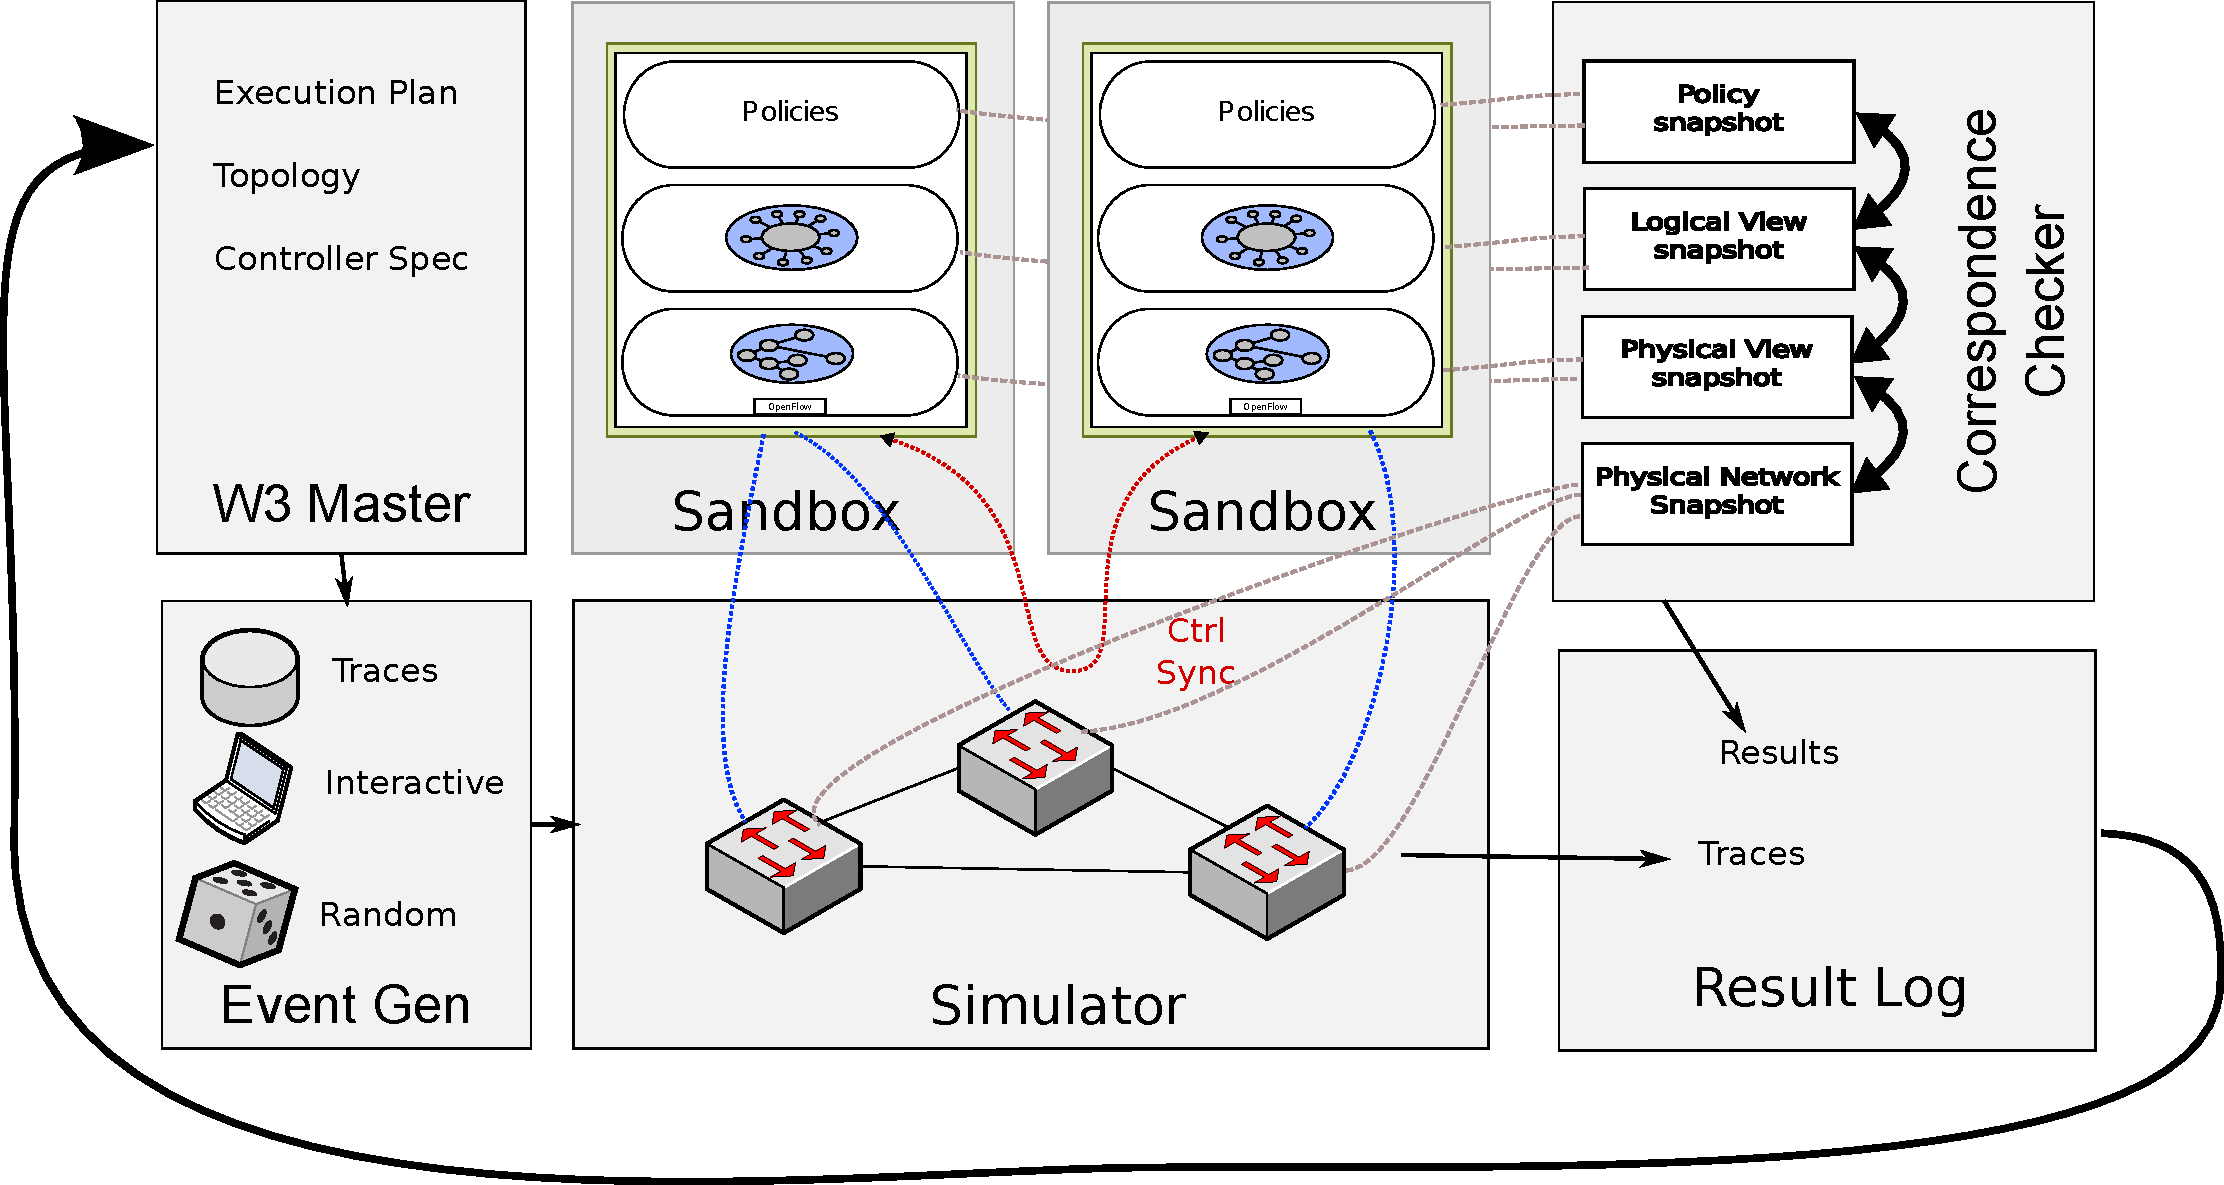
\includegraphics[width=0.8\textwidth{}]{../diagrams/architecture/architecture.pdf}
  \caption{System architecture. \colin{Andi: can haz new diagram? :P}}
  \label{fig:system}
\end{figure*}

\noindent{\bf Trace Input And Fuzzing.} Since a major goal of \projectname{} was
to support a wide range of usage scenarios, % WAT does that even mean
we provide support for three different methods for generating network trace
inputs. The most common method is to insert failure and topology change logs
from production deployments into the simulator for replay. Input traces may
also be produced synthetically with configurable, random probabilities for
network events. Lastly, we support interactive use, where the troubleshooter
has complete control over network events, and is thereby free to explore her
intuitions in order to reproduce a failure mode she has in mind.

\noindent{\bf Simulator.} We have built a simulator for SDN networks,
where network devices and hosts are modeled as lightweight python objects.
\colin{Reviewer OA: python objects creep in to the writing} Within a single thread, we
are able to deterministically model the execution of very large networks.
Our simulated model supports a wide
range of failure modes, and provides fine-grained control over event
orderings, component failures, and other aspects of the system execution. Our
simulator currently supports switch failures, link failures, arbitrary packet
re-orderings, drops and delays, and a fully general control plane.

The main challenge we encountered in the design of the simulator was
maintaining large numbers of TCP connections to the
controller(s). Although the controllers themselves may be spread
over multiple physical servers, the main simulator must nonetheless handle all
TCP connections between switches and controllers within a single process.
We ultimately ended up using epoll to avoid limitations of the UNIX select
implementation.

\noindent{\bf Controller Sandbox.} One of our major goals for \projectname{}
was to be able to run any SDN controller on top of the platform, with minimal
code changes to the controllers themselves. In addition, control servers
running on top of the simulated network must support deterministic execution
for reproducible results.

Currently we run applications as UNIX processes outside of the simulator.
We note however that there are a number of approaches for achieving deterministic
replay for external software. For example: a software determinism layer (e.g.
deterministic random number generators \colin{Reviewer OA: Whenever I see
replay, I worry about dealing with nondeterminism and pseudorandom number
generators. It was not clear how you are dealing with these issues.}) is
extremely lightweight, but requires modifications to the external software;
binary rewriting does not require any modification to the external
software's source code, but incurs moderate performance overhead; and VMs
fully support deterministic replay, but only a relatively small number of VMs can be run
on a single machine. We hope to leverage this previous work in future versions
of \projectname{}. Nonetheless, our architecture does not prevent us from
running controllers on different physical
servers in case we encounter memory or CPU bottlenecks.

\noindent{\bf Correspondence Checking.}
\projectname{} leverages the Hassel library provided by HSA~\cite{hsa}
to implement the correspondence checking algorithm. We optimize the code
slightly to run efficiently on large networks; in particular, we parallelize
symbolic packet propagation to a large number of subtasks. Correspondence
checking currently requires a small code change to the controller to fetch
the platform's view of the network state.

\projectname{} is written in roughly 10,000 lines of python, and is publicly
available. [anon]

}
